%%%%%%%%%%%%%%%%%%%%%%%%%%%%%%%%%%%%%%%%%%%%%%%%%%%%%%%%%%%%%%%%%%%%%%%%%%%%
% AGUtmpl.tex: this template file is for articles formatted with LaTeX2e,
% Modified December 2018
%
% This template includes commands and instructions
% given in the order necessary to produce a final output that will
% satisfy AGU requirements.
%
% FOR FIGURES, DO NOT USE \psfrag
%
%%%%%%%%%%%%%%%%%%%%%%%%%%%%%%%%%%%%%%%%%%%%%%%%%%%%%%%%%%%%%%%%%%%%%%%%%%%%
%
% IMPORTANT NOTE:
%
% SUPPORTING INFORMATION DOCUMENTATION IS NOT COPYEDITED BEFORE PUBLICATION.
%
%
%
%%%%%%%%%%%%%%%%%%%%%%%%%%%%%%%%%%%%%%%%%%%%%%%%%%%%%%%%%%%%%%%%%%%%%%%%%%%%
%
% Step 1: Set the \documentclass
%
%
% PLEASE USE THE DRAFT OPTION TO SUBMIT YOUR PAPERS.
% The draft option produces double spaced output.
%
% Choose the journal abbreviation for the journal you are
% submitting to:

% jgrga JOURNAL OF GEOPHYSICAL RESEARCH (use for all of them)
% gbc   GLOBAL BIOCHEMICAL CYCLES
% grl   GEOPHYSICAL RESEARCH LETTERS
% pal   PALEOCEANOGRAPHY
% ras   RADIO SCIENCE
% rog   REVIEWS OF GEOPHYSICS
% tec   TECTONICS
% wrr   WATER RESOURCES RESEARCH
% gc    GEOCHEMISTRY, GEOPHYSICS, GEOSYSTEMS
% sw    SPACE WEATHER
% ms    JAMES
% ef    EARTH'S FUTURE
%
%
%
% (If you are submitting to a journal other than jgrga,
% substitute the initials of the journal for "jgrga" below.)

\documentclass[draft,wrr]{agutexSI2019}

%%%%%%%%%%%%%%%%%%%%%%%%%%%%%%%%%%%%%%%%%%%%%%%%%%%%%%%%%%%%%%%%%%%%%%%%%
%
%  SUPPORTING INFORMATION TEMPLATE
%
%% ------------------------------------------------------------------------ %%
%
%
%Please use this template when formatting and submitting your Supporting Information.

%This template serves as both a “table of contents” for the supporting information for your article and as a summary of files.
%
%
%OVERVIEW
%
%Please note that all supporting information will be peer reviewed with your manuscript. It will not be copyedited if the paper is accepted.
%In general, the purpose of the supporting information is to enable authors to provide and archive auxiliary information such as data tables, method information, figures, video, or computer software, in digital formats so that other scientists can use it.
%The key criteria are that the data:
% 1. supplement the main scientific conclusions of the paper but are not essential to the conclusions (with the exception of
%    including %data so the experiment can be reproducible);
% 2. are likely to be usable or used by other scientists working in the field;
% 3. are described with sufficient precision that other scientists can understand them, and
% 4. are not exe files.
%
%USING THIS TEMPLATE
%
%***All references should be included in the reference list of the main paper so that they can be indexed, linked, and counted as citations.  The reference section does not count toward length limits.
%
%All Supporting text and figures should be included in this document. Insert supporting information content into each appropriate section of the template. To add additional captions, simply copy and paste each sample as needed.

%Tables may be included, but can also be uploaded separately, especially if they are larger than 1 page, or if necessary for retaining table formatting. Data sets, large tables, movie files, and audio files should be uploaded separately. Include their captions in this document and list the file name with the caption. You will be prompted to upload these files on the Upload Files tab during the submission process, using file type “Supporting Information (SI)”

%IMPORTANT NOTE ON FIGURES AND TABLES
% Placeholders for figures and tables appear after the \end{article} command, after references.
% DO NOT USE \psfrag or \subfigure commands.
%
 \usepackage{graphicx}
%
%  Uncomment the following command to allow illustrations to print
%   when using Draft:
 \setkeys{Gin}{draft=false}
%
% You may need to use one of these options for graphicx depending on the driver program you are using.
%
% [xdvi], [dvipdf], [dvipsone], [dviwindo], [emtex], [dviwin],
% [pctexps],  [pctexwin],  [pctexhp],  [pctex32], [truetex], [tcidvi],
% [oztex], [textures]
%
%
%% ------------------------------------------------------------------------ %%
%
%  ENTER PREAMBLE
%
%% ------------------------------------------------------------------------ %%

% Author names in capital letters:
%\authorrunninghead{BALES ET AL.}

% Shorter version of title entered in capital letters:
%\titlerunninghead{SHORT TITLE}

%Corresponding author mailing address and e-mail address:
%\authoraddr{Corresponding author: A. B. Smith,
%Department of Hydrology and Water Resources, University of
%Arizona, Harshbarger Building 11, Tucson, AZ 85721, USA.
%(a.b.smith@hwr.arizona.edu)}

\begin{document}

%% ------------------------------------------------------------------------ %%
%
%  TITLE
%
%% ------------------------------------------------------------------------ %%

%\includegraphics{agu_pubart-white_reduced.eps}


\title{Supporting Information for "Geometric models overestimate lake depth due to imperfect slope
measurement"}
%
% e.g., \title{Supporting Information for "Terrestrial ring current:
% Origin, formation, and decay $\alpha\beta\Gamma\Delta$"}
%
%DOI: 10.1002/%insert paper number here%

%% ------------------------------------------------------------------------ %%
%
%  AUTHORS AND AFFILIATIONS
%
%% ------------------------------------------------------------------------ %%


% List authors by first name or initial followed by last name and
% separated by commas. Use \affil{} to number affiliations, and
% \thanks{} for author notes.
% Additional author notes should be indicated with \thanks{} (for
% example, for current addresses).

% Example: \authors{A. B. Author\affil{1}\thanks{Current address, Antartica}, B. C. Author\affil{2,3}, and D. E.
% Author\affil{3,4}\thanks{Also funded by Monsanto.}}

\authors{J. Stachelek\affil{1}, P. J. Hanly\affil{1}, and P. A. Soranno\affil{1}}

\affiliation{1}{Department of Fisheries and Wildlife, Michigan State University, 480
Wilson Rd., East Lansing, MI 48824, USA}

% \affiliation{1}{First Affiliation}
% \affiliation{2}{Second Affiliation}
% \affiliation{3}{Third Affiliation}
% \affiliation{4}{Fourth Affiliation}

% \affiliation{=number=}{=Affiliation Address=}
%(repeat as many times as is necessary)





%% ------------------------------------------------------------------------ %%
%
%  BEGIN ARTICLE
%
%% ------------------------------------------------------------------------ %%

% The body of the article must start with a \begin{article} command
%
% \end{article} must follow the references section, before the figures
%  and tables.

\begin{article}

%% ------------------------------------------------------------------------ %%
%
%  TEXT
%
%% ------------------------------------------------------------------------ %%



\noindent\textbf{Contents of this file}
%%%Remove or add items as needed%%%
\begin{enumerate}

\item \textbf{Figure S1:} Diagram showing expectations regarding depth prediction bias

\item \textbf{Figure S2:} Hypsography classification by state

\item \textbf{Figure S3:} Lake geometry comparison among shape and reservoir classes

\item \textbf{Figure S4:} Lake geometry comparison among shape classes by depth and area

\item \textbf{Figure S5:} Effect of calculation technique on in-lake/nearshore slope comparison.

\item \textbf{Figure S6:} Importance plot for random forest variables

\item \textbf{Figure S7:} Characteristics of lakes with bathymetry versus non-bathymetry lakes

\item \textbf{Figure S8:} Lake characteristics comparison among shape and reservoir classes

\item \textbf{Figure S9:} Comparison between reported depth and bathymetry depth

\item \textbf{Table S1:} Summary of lake characteristics for the present study

\item \textbf{Table S2:} Effect of calculation technique on depth model fit and accuracy.

%if Tables are larger than 1 page, upload as separate excel file
\end{enumerate}
\vspace{1em}

% \noindent\textbf{Introduction}
%Type or paste your text here. The introduction gives a brief overview of the supporting information. You should include information %about as many of the following as possible (when appropriate):
% 1. a general overview of the kind of data files;
% 2. information about when and how the data were collected or created;
% 3. a general description of processing steps used;
% 4. any known imperfections or anomalies in the data.

%\clearpage

%Delete all unused file types below. Copy/paste for multiples of each file type as needed.
%\noindent\textbf{Text S1.}
%Type or paste text here. This should be additional explanatory text, such as: extended descriptions of results, full details of models, extended lists of acknowledgements etc.  It should not be additional discussion, analysis, interpretation or critique. It should not be an additional scientific experiment or paper.
%
%Repeat for any additional Supporting Text

%%Enter Data Set, Movie, and Audio captions here
%%EXAMPLE CAPTIONS

% \noindent\textbf{Data Set S1.} %Type or paste caption here.
%upload your dataset(s) to AGU's journal submission site and select "Supporting Information (SI)" as the file type. Following naming %convention: ds01.

%Repeat for any additional Supporting data sets

% \noindent\textbf{Movie S1.} %Type or paste caption here.
%upload your movie(s) to AGU's journal submission site and select, "Supporting Information %(SI)" as the file type. Following naming convention: ms01.

%Repeat any additional Supporting movies

% \noindent\textbf{Audio S1.} %Type or paste caption here.
%upload your audio file(s) to AGU's journal submission site and select "Supporting Information %(SI)" as the file type. Following naming convention: auds01.


%Repeat for any additional Supporting audio files

%%% End of body of article:
%%%%%%%%%%%%%%%%%%%%%%%%%%%%%%%%%%%%%%%%%%%%%%%%%%%%%%%%%%%%%%%%
%
% Optional Notation section goes here
%
% Notation -- End each entry with a period.
% \begin{notation}
% Term & definition.\\
% Second term & second definition.\\
% \end{notation}
%%%%%%%%%%%%%%%%%%%%%%%%%%%%%%%%%%%%%%%%%%%%%%%%%%%%%%%%%%%%%%%%


%% ------------------------------------------------------------------------ %%
%%  REFERENCE LIST AND TEXT CITATIONS

%%%%%%%%%%%%%%%%%%%%%%%%%%%%%%%%%%%%%%%%%%%%%%%
%
%
% \bibliography{lagosdepth}
%
% no need to specify bibliographystyle
%
% Note that ALL references in this supporting information file must also be referenced in the primary manuscript
%
%%%%%%%%%%%%%%%%%%%%%%%%%%%%%%%%%%%%%%%%%%%%%%%
% if you get an error about newblock being undefined, uncomment this line:
%\newcommand{\newblock}{}

% \bibliography{ uncomment this line and enter the name of your bibtex file here }




%Reference citation instructions and examples:
%
% Please use ONLY \cite and \citeA for reference citations.
% \cite for parenthetical references
% ...as shown in recent studies (Simpson et al., 2019)
% \citeA for in-text citations
% ...Simpson et al (2019) have shown...
% DO NOT use other cite commands (e.g., \citet, \citep, \citeyear, \nocite, \citealp, etc.).
%
%
%...as shown by \citeA{jskilby}.
%...as shown by \citeA{lewin76}, \citeA{carson86}, \citeA{bartoldy02}, and \citeA{rinaldi03}.
%...has been shown \cite<e.g.,>{jskilbye}.
%...has been shown \cite{lewin76,carson86,bartoldy02,rinaldi03}.
%...has been shown \cite{lewin76,carson86,bartoldy02,rinaldi03}.
%
% apacite uses < > for prenotes, not [ ]
% DO NOT use other cite commands (e.g., \citet, \citep, \citeyear, \nocite, \citealp, etc.).
%

%% ------------------------------------------------------------------------ %%
%
%  END ARTICLE
%
%% ------------------------------------------------------------------------ %%
\end{article}
\clearpage

\begin{figure}
      \begin{center}
        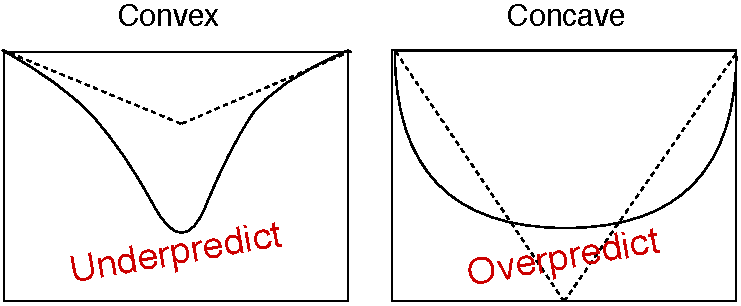
\includegraphics[width=0.75\textwidth,keepaspectratio]{../figures/lake_shape}
      \end{center}
      \caption{Diagram showing our expectation that slope-based models of lake depth will under predict true depth in convex lakes (left) and over predict true depth in concave lakes (right). Dashed lines represent extrapolated nearshore land slope while solid lines represent the lake bottom.}\label{figS1}
    \end{figure}

\clearpage

\begin{figure}
      \noindent\includegraphics[width=0.85\textwidth]{../figures/01_hypsography-1}
      \caption{Hypsography classification by state. Numbers on panel labels indicate the percentage of lakes in each state with a convex versus a concave cross-section shape.}\label{figS3}
      \end{figure}

\begin{figure}
      \noindent\includegraphics[width=0.85\textwidth]{../figures/01_geometry_grid-1}
      \caption{Comparison among lake shape and reservoir classes for A-B) distance to deepest point versus distance to lake visual center and C-D) nearshore slope versus inlake slope. A dashed 1:1 line is shown for comparison. Cross-section shape and reservoir class plots are not identical because not all lakes had a reservoir classification exceeding a 0.75 probability confidence level.}\label{figS4}
      \end{figure}

\begin{figure}
      \begin{center}
        \includegraphics[width=0.79\textwidth,keepaspectratio]{../figures/slope_by_area_depth-1}
      \end{center}
      \caption{Comparison between in-lake and nearshore slopes in concave and convex lakes of the same size and max depth.}\label{figS5}
    \end{figure}
\clearpage

\begin{figure}
      \begin{center}
        \includegraphics[width=\textwidth,keepaspectratio]{../figures/01_slope_compare-1}
      \end{center}
      \caption{Comparison between in-lake and nearshore slope using different calculation techniques. The techniques used in the main text analyses are bolded and the combination of these techniques (top-left corner) produces the strongest relationship between the two metrics. \texttt{slope\_mean} is the mean slope of all inlake or nearshore buffer points. \texttt{slope\_pnts} is the average slope (i.e. \texttt{slope\_pnt}) of all points at maximum depth. \texttt{slope\_online\_mean} is the mean pixel-to-pixel slope of each pixel lying on a straight line either from the single deepest point to the lake shoreline (in the case of inlake slope) or from the lake shoreline point extending to the buffer exterior (in the case of nearshore slope). \texttt{slopes\_online\_mean} is the same as \texttt{slope\_online\_mean} except it uses all inlake points at maximum depth.}\label{figS6}
    \end{figure}
\clearpage

\begin{figure}
      \noindent\includegraphics[width=0.85\textwidth]{../figures/02_depth_model_importance-1}
      \caption{Importance plot for random forest variables showing increase in mean square error. Higher values indicate greater importance to model predictions. See Equation 1 for a definition of geometric max depth. HUC4 ID is a 'dummy' variable of geographic (hydrologic subbasin) location.}\label{figS7}
      \end{figure}

\begin{figure}
      \begin{center}\includegraphics[width=0.45\textwidth]{../figures/gg_effort-1}\end{center}
            \caption{Comparison between characteristics of lakes with bathymetry data against lakes with depth from other sources in the LAGOSUS-Depth product. The distance to urban area metric is calculated using data from the 2018 US Census Urban and Rural Classification.}\label{figS8}
      \end{figure}

\clearpage
\begin{figure}
      \begin{center}\includegraphics[width=0.85\textwidth]{../figures/01_contrasts-1}\end{center}
      \caption{Comparison of lake characteristics according to differences in lake cross-section shape or reservoir status.}\label{figS9}
      \end{figure}

\clearpage

\begin{figure}
      \begin{center}\includegraphics[width=0.73\textwidth]{../figures/lgnemanual-vs-bathy-depth-1}\end{center}
      \caption{Comparison between reported depth and depth extracted from bathymetry surfaces by US State where reported depths come from the LAGOSUS-Depth product. For this figure, no reported depth values originated from the same source as its corresponding bathymetry-derived value.}\label{figS10}
      \end{figure}

\clearpage

% source at tables/01_predictors.Rmd
\begin{table}
\caption{Summary of lake characteristics for the present study (and for lakes in the contiguous United States). Predictor variables for computing random forest offsets (Equation 2) are printed in bold face. Dashes (-) indicate an identical sample size among this study and that of the contiguous United States.} \label{tableS1}
\centering
\setlength\tabcolsep{1.5pt} % default value: 6pt
\begin{tabular}{lllll}
\hline
Variable & Median & Q25 & Q75 & n\\
\hline
Max depth (m) & 8.2 (7) & 4.6 (3.7) & 14 (12) & 4820 (17700)\\
\textbf{Area (ha)} & 55 (33) & 21 (11) & 140 (100) & 4820 (17700)\\
\textbf{Island area (ha)} & 0 (0) & 0 (0) & 0.18 (0.076) & 4820 (17700)\\
\textbf{Perimeter (m)} & 4400 (3500) & 2500 (1800) & 8100 (7300) & 4820 (17700)\\
\textbf{Shoreline development} & 1.7 (1.7) & 1.4 (1.4) & 2.1 (2.2) & 4820 (17700)\\
\textbf{Elevation (m)} & 300 (340) & 180 (210) & 400 (460) & 4820 (17700)\\
\textbf{Watershed-lake ratio} & 7.8 (10) & 3.8 (4.4) & 17 (29) & 4820 (17700)\\
\textbf{Deepest point distance (m)} & 180 (-) & 110 (-) & 290 (-) & 4820 (-)\\
Mean deepest point distance (m) & 140 (-) & 87 (-) & 230 (-) & 4820 (-)\\
\textbf{Visual center distance (m)} & 240 (-) & 160 (-) & 390 (-) & 4820 (-)\\
Inlake slope (m/m) & 0.05 (-) & 0.02 (-) & 0.08 (-) & 4820 (-)\\
Inlake slope online (m/m) & 0.06 (-) & 0.03 (-) & 0.14 (-) & 4800 (-)\\
Inlake slopes (m/m) & 0.06 (-) & 0.03 (-) & 0.1 (-) & 4820 (-)\\
Inlake slopes online (m/m) & 0.07 (-) & 0.03 (-) & 0.15 (-) & 4800 (-)\\
Mean inlake slope (m/m) & 0.04 (-) & 0.02 (-) & 0.09 (-) & 4820 (-)\\
Nearshore mean slope (m/m) & 0.08 (-) & 0.05 (-) & 0.11 (-) & 4820 (-)\\
Nearshore slope online (m/m) & 0.08 (-) & 0.04 (-) & 0.13 (-) & 4590 (-)\\
Nearshore slopes online (m/m) & 0.08 (-) & 0.04 (-) & 0.13 (-) & 4540 (-)\\
\hline
\end{tabular}
\end{table}

\begin{table}
\caption{Model fit and predictive accuracy metrics (RMSE = root mean square error, $R^2$ = coefficient of determination, MAPE = mean absolute percent error) for the proxy - proxy combination of geometry metrics (see main text Table 1). Each row shows model metrics when proxy and "true" measures are calculated with slight differences from the default (bolded) used in the main text. \texttt{slope\_mean} is the mean slope of all inlake or nearshore buffer points. \texttt{slope\_pnts} is the average slope (i.e. \texttt{slope\_pnt}) of all points at maximum depth. \texttt{slope\_online\_mean} is the mean pixel-to-pixel slope of each pixel lying on a straight line either from the single deepest point to the lake shoreline (in the case of inlake slope) or from the lake shoreline point extending to the buffer exterior (in the case of nearshore slope). \texttt{slopes\_online\_mean} is the same as \texttt{slope\_online\_mean} except it uses all inlake points at maximum depth. \texttt{dists\_deepest} is the same as \texttt{dist\_deepest} except distance is calculated for all points at maximum depth.}  \label{tableS2}
\centering
\setlength\tabcolsep{1.5pt} % default value: 6pt
\begin{tabular}{lllllc}
\hline
Inlake slope & Nearshore slope & Inlake distance & RMSE & $R^2$ & MAPE\\
\hline
slope\_pnts & slope\_mean & dists\_deepest & 6.2 m & 0.38 & 58 \%\\
\textbf{slope\_pnt} & \textbf{slope\_mean} & \textbf{dist\_deepest} & \textbf{6.4 m} & \textbf{0.35} & \textbf{59 \%}\\
slope\_pnts & slopes\_online\_mean & dist\_deepest & 6.4 m & 0.32 & 61 \%\\
slope\_online\_mean & slope\_mean & dists\_deepest & 6.5 m & 0.41 & 63 \%\\
slope\_pnts & slope\_mean & dist\_deepest & 6.7 m & 0.44 & 58 \%\\
slope\_online\_mean & slope\_mean & dist\_deepest & 6.7 m & 0.36 & 59 \%\\
slope\_online\_mean & slopes\_online\_mean & dist\_deepest & 6.7 m & 0.32 & 66 \%\\
slope\_mean & slope\_mean & dists\_deepest & 6.8 m & 0.36 & 59 \%\\
slope\_pnt & slopes\_online\_mean & dists\_deepest & 6.8 m & 0.25 & 73 \%\\
slope\_pnts & slope\_online\_mean & dist\_deepest & 6.9 m & 0.3 & 71 \%\\
slope\_online\_mean & slope\_online\_mean & dist\_deepest & 6.9 m & 0.32 & 68 \%\\
slope\_online\_mean & slope\_online\_mean & dists\_deepest & 6.9 m & 0.33 & 65 \%\\
slope\_mean & slopes\_online\_mean & dists\_deepest & 7 m & 0.24 & 65 \%\\
slope\_mean & slope\_mean & dist\_deepest & 7.1 m & 0.4 & 64 \%\\
slopes\_online\_mean & slope\_mean & dist\_deepest & 7.1 m & 0.37 & 56 \%\\
slope\_mean & slope\_online\_mean & dist\_deepest & 7.1 m & 0.3 & 69 \%\\
slopes\_online\_mean & slopes\_online\_mean & dists\_deepest & 7.2 m & 0.32 & 63 \%\\
slopes\_online\_mean & slopes\_online\_mean & dist\_deepest & 7.3 m & 0.25 & 64 \%\\
slope\_pnt & slope\_mean & dists\_deepest & 7.3 m & 0.35 & 61 \%\\
slopes\_online\_mean & slope\_mean & dists\_deepest & 7.3 m & 0.36 & 60 \%\\
slope\_online\_mean & slopes\_online\_mean & dists\_deepest & 7.3 m & 0.29 & 58 \%\\
slope\_pnts & slope\_online\_mean & dists\_deepest & 7.4 m & 0.27 & 64 \%\\
slopes\_online\_mean & slope\_online\_mean & dists\_deepest & 7.4 m & 0.33 & 67 \%\\
slopes\_online\_mean & slope\_online\_mean & dist\_deepest & 7.5 m & 0.26 & 61 \%\\
slope\_pnt & slopes\_online\_mean & dist\_deepest & 7.5 m & 0.33 & 69 \%\\
slope\_mean & slopes\_online\_mean & dist\_deepest & 7.6 m & 0.26 & 64 \%\\
slope\_pnt & slope\_online\_mean & dist\_deepest & 7.7 m & 0.27 & 68 \%\\
slope\_pnts & slopes\_online\_mean & dists\_deepest & 7.8 m & 0.3 & 65 \%\\
slope\_pnt & slope\_online\_mean & dists\_deepest & 7.9 m & 0.27 & 67 \%\\
slope\_mean & slope\_online\_mean & dists\_deepest & 7.9 m & 0.31 & 60 \%\\
\hline
\end{tabular}
\end{table}

% Copy/paste for multiples of each file type as needed.

% enter figures and tables below here: %%%%%%%
%
%
%
%
% EXAMPLE FIGURES
% ---------------
% If you get an error about an unknown bounding box, try specifying the width and height of the figure with the natwidth and natheight options.
% \begin{figure}
%\setfigurenum{S1} %%You can change number for each figure if you want, not required. "S" prepended automatically.
% \noindent\includegraphics[natwidth=800px,natheight=600px]{samplefigure.eps}
%\caption{caption}
%\label{epsfiguresample}
%\end{figure}
%
%
% Giving latex a width will help it to scale the figure properly. A simple trick is to use \textwidth. Try this if large figures run off the side of the page.
% \begin{figure}
% \noindent\includegraphics[width=\textwidth]{anothersample.png}
%\caption{caption}
%\label{pngfiguresample}
%\end{figure}
%
%
%\begin{figure}
%\noindent\includegraphics[width=\textwidth]{athirdsample.pdf}
%\caption{A pdf test figure}
%\label{pdffiguresample}
%\end{figure}
%
% PDFLatex does not seem to be able to process EPS figures. You may want to try the epstopdf package.
%
%
% ---------------
% EXAMPLE TABLE
%
%\begin{table}
%\settablenum{S1} %%Change number for each table
%\caption{Time of the Transition Between Phase 1 and Phase 2\tablenotemark{a}}
%\centering
%\begin{tabular}{l c}
%\hline
% Run  & Time (min)  \\
%\hline
%  $l1$  & 260   \\
%  $l2$  & 300   \\
%  $l3$  & 340   \\
%  $h1$  & 270   \\
%  $h2$  & 250   \\
%  $h3$  & 380   \\
%  $r1$  & 370   \\
%  $r2$  & 390   \\
%\hline
%\end{tabular}
%\tablenotetext{a}{Footnote text here.}
%\end{table}
% ---------------
%
% EXAMPLE LARGE TABLE (UPLOADED SEPARATELY)
%\begin{table}
%\settablenum{S1} %%Change number for each table
%\caption{Time of the Transition Between Phase 1 and Phase 2\tablenotemark{a}}
%\end{table}


\end{document}

%%%%%%%%%%%%%%%%%%%%%%%%%%%%%%%%%%%%%%%%%%%%%%%%%%%%%%%%%%%%%%%

% More Information and Advice:

%% ------------------------------------------------------------------------ %%
%
%  SECTION HEADS
%
%% ------------------------------------------------------------------------ %%

% Capitalize the first letter of each word (except for
% prepositions, conjunctions, and articles that are
% three or fewer letters).

% AGU follows standard outline style; therefore, there cannot be a section 1 without
% a section 2, or a section 2.3.1 without a section 2.3.2.
% Please make sure your section numbers are balanced.
% ---------------
% Level 1 head
%
% Use the \section{} command to identify level 1 heads;
% type the appropriate head wording between the curly
% brackets, as shown below.
%
%An example:
%\section{Level 1 Head: Introduction}
%
% ---------------
% Level 2 head
%
% Use the \subsection{} command to identify level 2 heads.
%An example:
%\subsection{Level 2 Head}
%
% ---------------
% Level 3 head
%
% Use the \subsubsection{} command to identify level 3 heads
%An example:
%\subsubsection{Level 3 Head}
%
%---------------
% Level 4 head
%
% Use the \subsubsubsection{} command to identify level 3 heads
% An example:
%\subsubsubsection{Level 4 Head} An example.
%
%% ------------------------------------------------------------------------ %%
%
%  IN-TEXT LISTS
%
%% ------------------------------------------------------------------------ %%
%
% Do not use bulleted lists; enumerated lists are okay.
% \begin{enumerate}
% \item
% \item
% \item
% \end{enumerate}
%
%% ------------------------------------------------------------------------ %%
%
%  EQUATIONS
%
%% ------------------------------------------------------------------------ %%

% Single-line equations are centered.
% Equation arrays will appear left-aligned.

% Math coded inside display math mode \[ ...\]
%  will not be numbered, e.g.,:
%  \[ x^2=y^2 + z^2\]
%
%  Math coded inside \begin{equation} and \end{equation} will
%  be automatically numbered, e.g.,:
%  \begin{equation}
%  x^2=y^2 + z^2
%  \end{equation}

% IF YOU HAVE MULTI-LINE EQUATIONS, PLEASE
% BREAK THE EQUATIONS INTO TWO OR MORE LINES
% OF SINGLE COLUMN WIDTH (20 pc, 8.3 cm)
% using double backslashes (\\).

% To create multiline equations, use the
% \begin{eqnarray} and \end{eqnarray} environment
% as demonstrated below.
% \begin{eqnarray}
%   x_{1} & = & (x - x_{0}) \cos \Theta \nonumber \\
%         && + (y - y_{0}) \sin \Theta  \nonumber \\
%   y_{1} & = & -(x - x_{0}) \sin \Theta \nonumber \\
%         && + (y - y_{0}) \cos \Theta.
% \end{eqnarray}

%If you don't want an equation number, use the star form:
%\begin{eqnarray*}...\end{eqnarray*}

% Break each line at a sign of operation
% (+, -, etc.) if possible, with the sign of operation
% on the new line.

% Indent second and subsequent lines to align with
% the first character following the equal sign on the
% first line.

% Use an \hspace{} command to insert horizontal space
% into your equation if necessary. Place an appropriate
% unit of measure between the curly braces, e.g.
% \hspace{1in}; you may have to experiment to achieve
% the correct amount of space.


%% ------------------------------------------------------------------------ %%
%
%  EQUATION NUMBERING: COUNTER
%
%% ------------------------------------------------------------------------ %%

% You may change equation numbering by resetting
% the equation counter or by explicitly numbering
% an equation.

% To explicitly number an equation, type \eqnum{}
% (with the desired number between the brackets)
% after the \begin{equation} or \begin{eqnarray}
% command.  The \eqnum{} command will affect only
% the equation it appears with; LaTeX will number
% any equations appearing later in the manuscript
% according to the equation counter.
%

% If you have a multiline equation that needs only
% one equation number, use a \nonumber command in
% front of the double backslashes (\\) as shown in
% the multiline equation above.

%% ------------------------------------------------------------------------ %%
%
%  SIDEWAYS FIGURE AND TABLE EXAMPLES
%
%% ------------------------------------------------------------------------ %%
%
% For tables and figures, add \usepackage{rotating} to the paper and add the rotating.sty file to the folder.
% AGU prefers the use of {sidewaystable} over {landscapetable} as it causes fewer problems.
%
% \begin{sidewaysfigure}
% \includegraphics[width=20pc]{samplefigure.eps}
% \caption{caption here}
% \label{label_here}
% \end{sidewaysfigure}
%
%
%
% \begin{sidewaystable}
% \caption{}
% \begin{tabular}
% Table layout here.
% \end{tabular}
% \end{sidewaystable}
%
%

